\documentclass[11pt,oneside,openright]{./style/phdthesis}

\usepackage{amsmath}
\usepackage[ansinew]{inputenc}
\usepackage[portuguese]{babel}
\usepackage[printonlyused, withpage]{acronym}
\usepackage{a4wide}
\usepackage{palatino}
\usepackage{fancyhdr}
\usepackage{fancybox}
\usepackage{amssymb}
%\usepackage{chapterbib} %com este package as referencias bibliográficas aparecem no final de cada capítulo
\usepackage{cite}
\usepackage{epsfig}
\usepackage{subfigure}
\usepackage{graphics}
\usepackage{float}
\usepackage{here}
\usepackage[T1]{fontenc}
\usepackage{rotating}
\usepackage{multirow}
%\usepackage{comment}
%\usepackage{captionhack}
\usepackage{epigraph}
\usepackage[linkcolor=black]{hyperref}
%\renewcommand{\thesubfigure}{}
\hypersetup{colorlinks=true}
\usepackage{enumerate}
%\usepackage[numbers,sort&compress]{natbib}
%\usepackage{hypernat}
\usepackage{booktabs}
\usepackage{url}                    % needed to cite a site
\usepackage{eurosym}
\usepackage{makeidx}
\usepackage{datatool}
\usepackage[toc, acronym]{glossaries}
\usepackage{graphicx}
\usepackage{caption}
%\usepackage{subcaption}

\usepackage{tabulary}
\usepackage{braket}

% subfile handling packages
\usepackage{subfiles}

\usepackage{multicol}
\usepackage{tcolorbox}
\usepackage{booktabs}

\usepackage{pdfpages}               % to append pdf files \includepdf[pages={-}]{myfile.pdf}



\newcommand{\onlyinsubfile}[1]{#1}
\newcommand{\notinsubfile}[1]{}
\renewcommand{\textfraction}{0.01}
\renewcommand{\topfraction}{0.99}
\renewcommand{\floatpagefraction}{0.99}
\renewcommand{\bottomfraction}{0.99}
\renewcommand{\heavyrulewidth}{1pt}
\renewcommand{\lightrulewidth}{0.50pt}
\renewcommand{\chaptername}{Capítulo}
\renewcommand{\figurename}{Figura}
\renewcommand{\appendixname}{\Large{Anexo}}
\renewcommand{\tablename}{Tabela}
\renewcommand{\acronymname}{Acrónimos}

\newcommand{\mli}[1]{\mathit{#1}}
\newcommand{\intSpace}{\!\!\!\!}
\newcommand{\doubleInt}{\!\!\int\intSpace\int\!\!}
\newcommand{\TX}{\mathit{TX}}
\newcommand{\NLI}{\mathit{NLI}}
\newcommand{\eff}{\mathit{eff}}
\newcommand{\LOASE}{\mathit{LO-ASE}}
\newcommand{\LONLI}{\mathit{LO-NLI}}
\renewcommand{\kbldelim}{[}% Left delimiter
\renewcommand{\kbrdelim}{]}% Right delimiter

%\makesavenoteenv{tabular}



\hyphenpenalty=50000
\tolerance=10000
%%% General page formatting

\oddsidemargin 0.2in
\evensidemargin 0in
%\textwidth 155mm
\headheight 15.0pt
\topmargin 0in
%\textheight 237mm

% footheight 1.0in

\makeatletter
\providecommand*{\diff}%
{\@ifnextchar^{\DIfF}{\DIfF^{}}}
\def\DIfF^#1{%
\mathop{\mathrm{\mathstrut d}}%
\nolimits^{#1}\gobblespace}
\def\gobblespace{%
\futurelet\diffarg\opspace}
\def\opspace{%
\let\DiffSpace\!%
\ifx\diffarg(%
\let\DiffSpace\relax
\else
\ifx\diffarg[%
\let\DiffSpace\relax
\else
\ifx\diffarg\{%
\let\DiffSpace\relax
\fi\fi\fi\DiffSpace}

\providecommand*{\tDeriv}[3][]{%
\frac{\diff^{#1}#2}{\diff #3^{#1}}}
\providecommand*{\pDeriv}[3][]{%
\frac{\partial^{#1}#2}%
{\partial #3^{#1}}}

\graphicspath{{./figures/}}


\DeclareMathOperator{\erf}{erf}
\DeclareMathOperator{\erfc}{erfc}
\DeclareMathOperator{\sinc}{sinc}
\DeclareMathOperator{\R}{Re}
\DeclareMathOperator{\I}{Im}
\DeclareMathOperator{\asinh}{asinh}

%\newcommand{\publ}{}

\pagenumbering{arabic} 


\makeindex

\begin{document}
%%  include the LaTeX files containing the text for each chapters

% ------------------------------------------------------------------------
\title{NetXPTO - NetPlanner}
\author{}
\date{\today}
\maketitle
% ------------------------------------------------------------------------

% ------------------------------------------------------------------------
\tableofcontents
% ------------------------------------------------------------------------


\chapter{Introduction}
\label{introduction}

The amount of traffic, in particular IP traffic, has been increasing very substantially. This increase is due to the growing number of Internet-based applications, the increase in the number of devices connected to the Internet, the expansion of optical fiber to customers' homes, increased bandwidth of mobile access technologies, and increased of video traffic.
At the same time, with the increase in traffic, operators are under heavy pressure to reduce the cost per bit transported. This implies the introduction of new technologies, which on the one hand increase the capacity of transport of the networks and on the other, reduce the costs of operation (OPEX).
This process of technological conversion is operating in a macroeconomic scenario in which operators find it difficult to finance which forces them to have strong investment constraints (CAPEX).
The transport networks have been networks predominantly based on circuit switching, either at the level of the optical channels or at the level of the electrical circuits, and the introduction of packet switching undermines this paradigm.
In this scenario, particularly considering the increase in packet traffic, packet switching solutions for transport networks and mixed solutions have been presented by the device manufacturers where packet and circuit switching coexists on the same equipment.

\newpage
%%%%%%%%%%%%%%%%%%%%%%%%%%%%%%%%%%%%%%%%%%%%%%%%%%%%%%%%%%%%%%%%%%%%%%%%
\section{Motivation and objectives}
\label{objectives}
Falta motivação.

To achieve the main objectives of this dissertation, the following steps must be taken:

\begin{enumerate}
  \item Define one reference network and three different scenarios for performing tests.
  \item Develop ILP models for opaque, transparent and translucent networks without protection and using 1 + 1 protection.
  \item Develop ILP models for opaque, transparent and translucent networks with 1 + 1 protection.
  \item Get analytical solutions for the two previous points.
  \item Compare the analytical results and results based on ILP with the results obtained through heuristics.
\end{enumerate}


%%%%%%%%%%%%%%%%%%%%%%%%%%%%%%%%%%%%%%%%%%%%%%%%%%%%%%%%%%%%%%%%%%%%%%%%%%%%%%%%%%%%%%%
\section{Thesis outline}
\label{outline}

This thesis is organized in 7 chapters. Chapter \ref{chap_reference_network} consists of a state-of-art review about optical transport networks. In this chapter is also where the reference network used throughout the dissertation as well as the different traffics used is defined. The Chapter \ref{chap_capex} begins by determining the CAPEX calculation formula for use in the ILP model and for analytical calculations. The first section refers to ILP models and the other to analytical models. In Chapter \ref{chap_ilp} are several sections each for a particular mode of transport and certain survivability. In section \ref{ILP_Opaque_Survivability} we have opaque without survivability, in section \ref{ILP_Opaque_Protection} opaque with 1+1 protection. Sections \ref{ILP_Transp_Survivability} and \ref{ILP_Transp_Protection} relate to the transparent and lastly sections \ref{ILP_Transluc_Survivability} and \ref{ILP_Transluc_Protection} refer to the translucent. In the referred section it is possible to see the model description, the detailed description of the results and the conclusions of these results. The analytical calculation of all the models referred to in Chapter \ref{chap_ilp} can be found in Chapter \ref{chap_analytical}. In Chapter \ref{chap_comparative} the results obtained throughout this dissertation are compared and the chapter is divided into six sections where each corresponds to a certain mode of transport with their respective survivability. The last step is the conclusions \ref{chap_conclusions} and suggestions for future research directions.

%%%%%%%%%%%%%%%%%%%%%%%%%%%%%%%%%%%%%%%%%%%%%%%%%%%%%%%%%%%%%%%%%%%%%%%%%%%%%%%%%%%%%%%%%%%%%%%%%%%%%%%%%%%%%%%%%%%%%%%%%%%%%


% ------------------------------------------------------------------------
\chapter{Simulator Structure}

LinkPlanner is a signals open-source simulator.

The major entity is the system.

A system comprises a set of blocks.

The blocks interact with each other through signals.

\section{System}

\section{Blocks}

\section{Signals}

List of available signals:

\begin{itemize}
    \item Signal

\end{itemize}










% ------------------------------------------------------------------------
\chapter{Development Cycle}

The NetXPTO-LinkPlanner has been developed by several people using git as a version control system.
The NetXPTO-LinkPlanner repository is located in the GitHub site http://github.com/netxpto/linkplanner.
The more updated functional version of the software is in the branch master.
Master should be considered a functional beta version of the software.
Periodically new releases are delivered from the master branch under the branch name Release<Year><Month><Day>.
The integration of the work of all people is performed by Armando Nolasco Pinto in the branch Develop.
Each developer has is how branch with his/her name.





% ------------------------------------------------------------------------
\chapter{Case Studies}

\clearpage

\begin{tcolorbox}	
\begin{tabular}{p{2.75cm} p{0.2cm} p{10.5cm}} 	
\textbf{Student Name}  &:& Tiago Esteves\\
\textbf{Starting Date} &:& October 03, 2017\\
\textbf{Goal}          &:& Implement the dimensioning of optical networks in the translucent transport mode.
\end{tabular}
\end{tcolorbox}

\section{Opaque with 1+1 Protection}
In this case study we focus on the opaque case with 1 + 1 protection.

\subsection{Physical Network Topology}

\subsubsection{Reference Network}
As we can see in the figure, our reference network consists of 6 nodes and 8 Bidirectional links.
The average length of the links was chosen so that the following calculations are more simplistic.

\begin{figure}[h!]
\centering
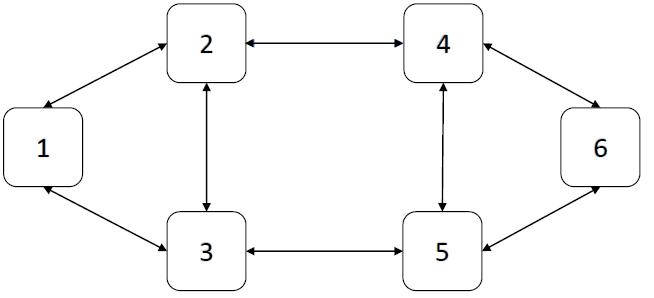
\includegraphics[width=\textwidth]{RedeTeste}
\caption{Physical Topology of the Reference Network.}
\end{figure}


The following table shows the values of the variables associated with this network.
\begin{table}[h!]
\centering
\begin{tabular}{|| c | c | c||}
 \hline
 Constant & Description & Value \\
 \hline\hline
 N & Number of Nodes & 6 \\
 L & Number of Bidirectional Links & 8 \\
 <$\delta$> & Node out-degree & 2,667 \\
 <len> & Mean Link Length (km) & 500 \\
 <h> & Mean Number of Hops,for Working Paths & 1,533 \\
 <h'> & Mean Number of Hops,for Backup Paths & 2,467 \\
 \hline
\end{tabular}
\caption{Table of reference network values}
\label{table:1}
\end{table}

As we can see from table \ref{table:1}, to do all the calculations necessary for this project, let us know the value of the traffic used. This value is defined depending on the scenario used, as we can see:
\begin{itemize}
  \item Low Traffic: \textbf{0.5 TBits/s}
  \item High Traffic: \textbf{5 TBits/s}
\end{itemize}

\subsubsection{Realistic Network}
The real network chosen for this work is the EON (European Optical Network).
The way the nodes are arranged geographically can be seen from the following figure.

\begin{figure}[h!]
\centering
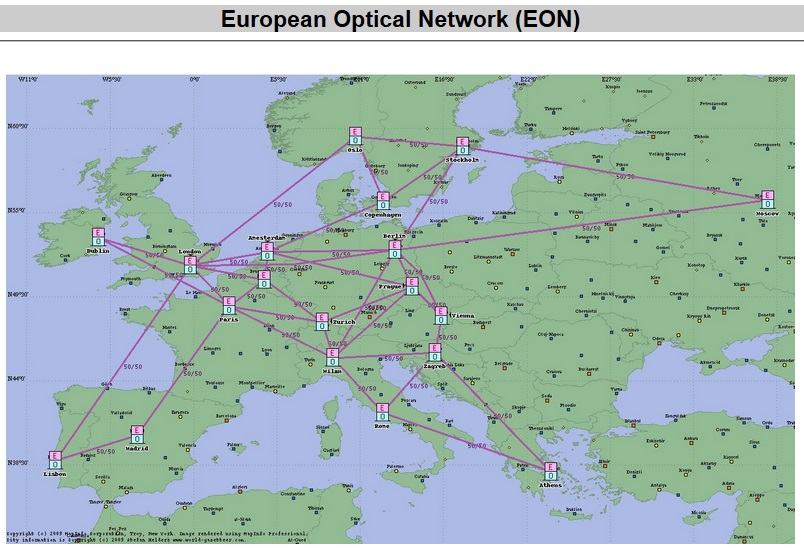
\includegraphics[width=\textwidth]{EON_Rede_Realista}
\caption{Physical Topology of the Realistic Network.}
\end{figure}

\begin{table}[h!]
The table \ref{table:2} shows the values of the variables associated with this network.\vspace{10pt}
\centering
\begin{tabular}{|| c | c | c||}
 \hline
 Constant & Description & Value \\
 \hline\hline
 N & Number of Nodes & 19 \\
 L & Number of Bidirectional Links & 37 \\
 <$\delta$> & Node out-degree & 3,89 \\
 <len> & Mean Link Length (km) & 753,76 \\
 <h> & Mean Number of Hops,for Working Paths & 2,3 \\
 <h'> & Mean Number of Hops,for Backup Paths & 3,2 \\
 \hline
\end{tabular}
\caption{Table of realistic network values}
\label{table:2}
\end{table}

Again, to make all the necessary calculations, only the value of the traffic used is missing. This value is set depending on the scenario used, as we can see:

\begin{itemize}
  \item Low Traffic: \textbf{2 TBits/s}
  \item High Traffic: \textbf{20 TBits/s}
\end{itemize}

\subsection{Dimensioning using ILP}

\subsubsection{ILP models}\label{ILP_models_OP}
The objective function of following ILP is a minimization of the sum of two variables: total number of flows crossing link (i; j) for all demand pairs (o; d) and total number of optical channels in each link (i; j).

\begin{equation}
minimize    \sum_{(i,j)} \sum_{(o,d)} f_{ij}^{od} + \sum_{(i,j)} W_{ij}
\label{ILPOpaque}
\end{equation}

$subject$ $to$
\begin{equation}
\sum_{j\textbackslash \{o\}} f_{ij}^{od} = 2  \qquad \qquad \qquad \qquad \qquad \qquad \qquad \qquad \qquad \qquad
\forall(o,d) : o < d, \forall i: i = o
\label{ILPOpaque1}
\end{equation}

\vspace{-5pt}
\begin{equation}
\sum_{j\textbackslash \{o\}} f_{ij}^{od} = \sum_{j\ \{d\}} f_{ji}^{od}   \qquad \qquad \qquad \qquad \qquad \qquad \qquad \qquad
\forall(o,d) : o < d, \forall i: i \neq o,d
\label{ILPOpaque2}
\end{equation}

\vspace{-5pt}
\begin{equation}
\sum_{j\textbackslash \{d\}} f_{ji}^{od} = 2  \qquad \qquad \qquad \qquad \qquad \qquad \qquad \qquad \qquad \qquad
\forall(o,d) : o < d, \forall i: i = d
\label{ILPOpaque3}
\end{equation}

\vspace{-5pt}
\begin{equation}
\sum_{(o,d):o<d} \left(f_{ij}^{od} + f_{ji}^{od}\right) + \sum_{c\in C} (B\left(c\right) D_{cod}\leq100 W_{ij} G_{ij} \qquad \qquad \qquad \qquad \qquad
\forall(i,j) : i < j
\label{ILPOpaque4}
\end{equation}

\vspace{-5pt}
\begin{equation}
W_{ij} \leq 80 \qquad  \qquad \qquad \qquad \qquad \qquad \qquad \qquad \qquad \qquad \qquad \qquad \qquad \forall(i,j) : i < j
\label{ILPOpaque5}
\end{equation}

\vspace{-5pt}
\begin{equation}
f_{ij}^{od} , f_{ji}^{od} \in \{0,2\}   \qquad \qquad \qquad \qquad \qquad \qquad \qquad \qquad \qquad
\forall(i,j) : i < j, \forall(o,d) : o < d
\label{ILPOpaque6}
\end{equation}

\vspace{-5pt}
\begin{equation}
W_{ij} \in \mathbb{N}  \qquad \qquad \qquad \qquad \qquad \qquad \qquad \qquad \qquad \qquad \qquad \qquad \qquad
\forall(i,j) : i < j\label{ILPOpaque7}
\end{equation}


The objective function, to be minimized, is the expression \ref{ILPOpaque}. The flow conservation constraints are \ref{ILPOpaque1}, \ref{ILPOpaque2} and \ref{ILPOpaque3}. First constraint ensures that, for all demand pairs (o,d), it routes two flows of traffic for all bidirectional links (i,j) when $j$ is not equal to the origin of the demand. Equation \ref{ILPOpaque3} is based on the same idea of \ref{ILPOpaque}, however applied in reverse direction. Assuming bidirectional traffic, so the number of flows in both directions of the link is the same \ref{ILPOpaque2}. The inequality \ref{ILPOpaque4} is considered grooming constraint, so it means the total client traffic flows can not be greater than the capacity of optical channels on all links. Another important constraint \ref{ILPOpaque5} is the capacity of the optical channels which must be less or equal to 100 Gb/s or 80 ODU0. The number of flows per demand can be zero if there are no traffic demands or two if considering working and protection traffic \ref{ILPOpaque6}. The last constraint is just needed to ensure the number optical of channels is a positive integer values greater than zero.


\subsubsection{ILP Results}

In this initial phase the results will be presented using ILP to calculate the CAPEX of the reference network.

The value of the CAPEX of the network will be calculated based on the costs of the equipment present in the figure below.
\begin{figure}[h!]
  \centering
  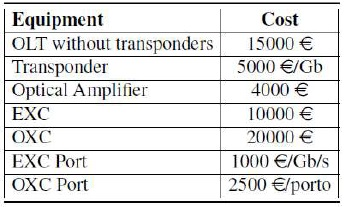
\includegraphics[scale=1]{TabValor}
  \caption{Table with costs}
  \label{TabCustOp}
\end{figure}

In addition to the equipment costs, we will also use the parameter "span", which in this case will have a value of 100.
Because this value is used to calculate the number of optical amplifiers required in the network using Equation \ref{amplifiers}.

\begin{equation}
N^R = \sum\limits_{l=1}^L\left(\left\lceil\frac{len_l}{span}\right\rceil-1\right)
\label{amplifiers}
\end{equation}

The other parameters of this equation are:
\begin{itemize}
\item{$N^R$			$\rightarrow$ Total number of regenerators/amplifiers}
\item{$len_l$		$\rightarrow$ Length of link l}
\item{$span$		$\rightarrow$ Distance between amplifiers}	
\end{itemize}	

To know the value of CAPEX it is necessary to know the value of the cost of the links and the cost of the nodes.

To calculate the cost of the nodes, the sum of the costs of the optical and electrical node is made. For this case the value of the optical cost is zero only needing to know the electric cost of the nodes that is given by equation \ref{electricalCostOpaque}.

\begin{equation}
C_{exc} = \left(\gamma_{e0}\times N\right) + \gamma_{e1} \times \left(T_1 + \left(2 \times w^0 \times \tau \right)\right)
\label{electricalCostOpaque}
\end{equation}

\begin{itemize}
\item{$C_{exc}$		$\rightarrow$	Electrical Ports Cost}
\item{$\gamma_{e0}$	$\rightarrow$	EXC cost in Euros}
\item{$N$			$\rightarrow$	Number of Nodes}
\item{$\gamma_{e1}$	$\rightarrow$	EXC port cost in Euros}
\item{$T_1$         $\rightarrow$   Total Unidirectional Traffic}
\item{$w^0$			$\rightarrow$	Total number of optical channels}
\item{$\tau$		$\rightarrow$	Traffic per port}
\end{itemize}

To calculate the cost of the Links we will use the equation \ref{linkCosts}.

\begin{equation}
C_L = \left(\gamma_0^{OLT} \times L\right) + \left(\gamma_1^{OLT} \times \tau \times W\right) + \left(N^R \times c^R\right)
\label{linkCosts}
\end{equation}	
	
\begin{itemize}
\item{$C_L$				$\rightarrow$	Links Cost}
\item{$\gamma_0^{OLT}$	$\rightarrow$	OLT cost in Euros}
\item{$L$				$\rightarrow$	Number of unidirectional Links}
\item{$\gamma_1^{OLT}$	$\rightarrow$	Transponder cost in Euros}
\item{$W$             $\rightarrow$	Total number of optical channels}
\item{$N^R$				$\rightarrow$	Total number of optical amplifiers}
\item{$c^R$				$\rightarrow$	Optical amplifiers cost in Euros}
\end{itemize}

To perform the calculations using the implementation of the models described in section \ref{ILP_models_OP} it is necessary to use a mathematical software tool. For this we will use MATLAB which is ideal for dealing with linear programming problems and can call the LPsolve through an external interface.

\pagebreak
Using the values calculated through MatLab as well as the values indicated in table \ref{table:1} or table \ref{table:2} (depending on the scenario used) and figure \ref{TabCustOp} we can finally calculate the CAPEX value using equations \ref{electricalCostOpaque} and \ref{linkCosts} for the various situations mentioned.\\

\textbf{Low Traffic scenario:}\\

$C_L$ = \textbf{24 336 000\euro}

$C_N$ = $C_{exc}$ = \textbf{5 860 000\euro}

$CAPEX$ = 24 336 000 + 5 860 000 = \textbf{30 196 000\euro}\\

\textbf{High Traffic scenario:}\\

$C_L$ = \textbf{191 336 000\euro}

$C_N$ = $C_{exc}$ = \textbf{48 260 000 \euro}

$CAPEX$ = 191 336 000 + 48 260 000 = \textbf{239 596 000 \euro}\\

\subsection{Dimensioning using Heuristics}

\subsubsection{Heuristics Models}

\subsubsection{Heuristics Results}

\subsection{Analysis and comparison of results}

\clearpage

\section{Transparent with 1+1 Protection}
In this case study we focus on the transparent case with 1 + 1 protection.
In this mode of transport, the information travels in a route defined through optical channels between origin and destination nodes always in the optical domain and, consequently, physical topology and logical topology are different.
An advantage of this mode of transport is the possibility of transporting express traffic.
An disadvantage is that the capacity utilization of the optical channels is worse than in the opaque mode of transport due to grooming only customer signs with the same endpoints.

\subsection{Physical Network Topology}
\begin{tcolorbox}	
\begin{tabular}{p{2.75cm} p{0.2cm} p{10.5cm}} 	
\textbf{Student Name}  &:& Tiago Esteves    (October 03, 2017 - )\\
\textbf{Goal}          &:& Implement the dimensioning of optical networks in the transparent transport mode.
\end{tabular}
\end{tcolorbox}
\vspace{-5pt}

\subsubsection{Reference Network}
In the figure below we ca see that our reference network consists of 6 nodes and 8 Bidirectional links.
The matrix of distances between the respective nodes and the ODU's matrices are the same as those reported in the opaque transport mode.

\begin{figure}[h!]
\centering
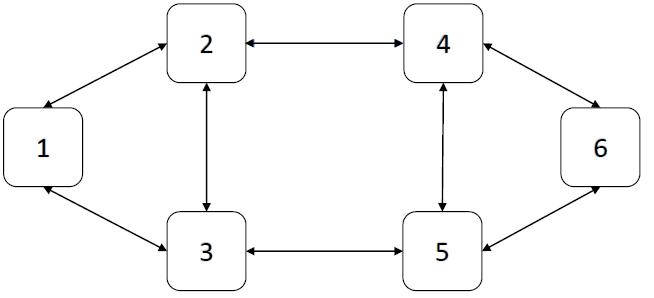
\includegraphics[width=\textwidth]{RedeTeste}
\caption{Physical Topology of the Reference Network.}
\end{figure}

The distance matrix is the same for the two scenarios but the ODU's matrices are not.
In this case only the matrices for the case of high traffic are elucidated, being that in the case of a low traffic it is only necessary to divide these matrices by the value 10.

\[
Dist=
  \begin{bmatrix}
    0 & 500 & 500 & 0 & 0 & 0 \\
    500 & 0 & 400 & 500 & 0 & 0 \\
    500 & 400 & 0 & 0 & 500 & 0 \\
    0 & 500 & 0 & 0 & 600 & 450 \\
    0 & 0 & 500 & 600 & 0 & 550 \\
    0 & 0 & 0 & 450 & 550 & 0
  \end{bmatrix}
\quad ODU0=
  \begin{bmatrix}
    0 & 50 & 10 & 30 & 10 & 30 \\
    50 & 0 & 0 & 10 & 50 & 0 \\
    10 & 0 & 0 & 10 & 40 & 10 \\
    30 & 10 & 10 & 0 & 10 & 0 \\
    10 & 50 & 40 & 10 & 0 & 30 \\
    30 & 0 & 10 & 10 & 30 & 0
  \end{bmatrix}
\]
\[
ODU1=
  \begin{bmatrix}
    0 & 20 & 40 & 20 & 0 & 50 \\
    20 & 0 & 0 & 30 & 10 & 10 \\
    40 & 0 & 0 & 10 & 10 & 0 \\
    30 & 30 & 10 & 0 & 10 & 30 \\
    0 & 10 & 10 & 10 & 0 & 10 \\
    50 & 10 & 0 & 30 & 10 & 0
  \end{bmatrix}
\quad ODU2=
  \begin{bmatrix}
    0 & 10 & 10 & 10 & 0 & 0 \\
    10 & 0 & 0 & 0 & 10 & 0 \\
    10 & 0 & 0 & 10 & 10 & 0 \\
    10 & 0 & 10 & 0 & 10 & 0 \\
    0 & 10 & 10 & 10 & 0 & 10 \\
    0 & 0 & 0 & 0 & 10 & 0
  \end{bmatrix}
\]
\[
ODU3=
  \begin{bmatrix}
    0 & 0 & 0 & 0 & 0 & 0 \\
    0 & 0 & 10 & 0 & 0 & 10 \\
    0 & 10 & 0 & 0 & 10 & 0 \\
    0 & 0 & 0 & 0 & 0 & 0 \\
    0 & 0 & 10 & 0 & 0 & 0 \\
    0 & 10 & 0 & 0 & 0 & 0
  \end{bmatrix}
\qquad ODU4=
  \begin{bmatrix}
    0 & 0 & 0 & 0 & 0 & 0 \\
    0 & 0 & 0 & 0 & 0 & 10 \\
    0 & 0 & 0 & 0 & 0 & 0 \\
    0 & 0 & 0 & 0 & 0 & 0 \\
    0 & 0 & 0 & 0 & 0 & 10 \\
    0 & 10 & 0 & 0 & 10 & 0
  \end{bmatrix}
\]

Through these ODU's we can calculate total network traffic for the low traffic scenario:\\
$T_1^0$ = 600x1.25 = 750 Gbits/s \qquad
$T_1^1$ = 500x2.5 = 1250 Gbits/s \qquad
$T_1^2$ = 160x10 = 1600 Gbits/s \\
$T_1^3$ = 60x40 = 2400 Gbits/s \quad
$T_1^4$ = 40x100 = 4000 Gbits/s \\
$T_{1total}$ = 750 + 1250 + 1600 + 2400 + 4000 = 10000 Gbits/s \qquad
$T_{total}$ = 10000/2 = 5 Tbits/s\\

We can thus conclude that the total traffic for the two scenarios is as follows:
\begin{itemize}
  \item Low Traffic: \textbf{0.5 TBits/s}
  \item High Traffic: \textbf{5 TBits/s}
\end{itemize}

Finally for this project has to take into consideration the table \ref{table:3} because in it we can see the values of the variables associated with this network.
\begin{table}[h!]
\centering
\begin{tabular}{|| c | c | c||}
 \hline
 Constant & Description & Value \\
 \hline\hline
 N & Number of nodes & 6 \\
 L & Number of bidirectional links & 8 \\
 <$\delta$> & Node out-degree & 2.667 \\
 <len> & Mean link length (km) & 500 \\
 <h> & Mean number of hops for working paths & 1.533 \\
 <h'> & Mean number of hops for backup paths & 2.467 \\
 \hline
\end{tabular}
\caption{Table of reference network values}
\label{table:3}
\end{table}


\subsubsection{Realistic Network}
The real network chosen for this work is the EON (European Optical Network).
The way the nodes are arranged geographically can be seen from the following figure and the matrix of distances created in the next page is constructed based on real distances.
In this case just ODU's matrices are created to be able to determine the total traffic used in each scenario.

\begin{figure}[h!]
\centering
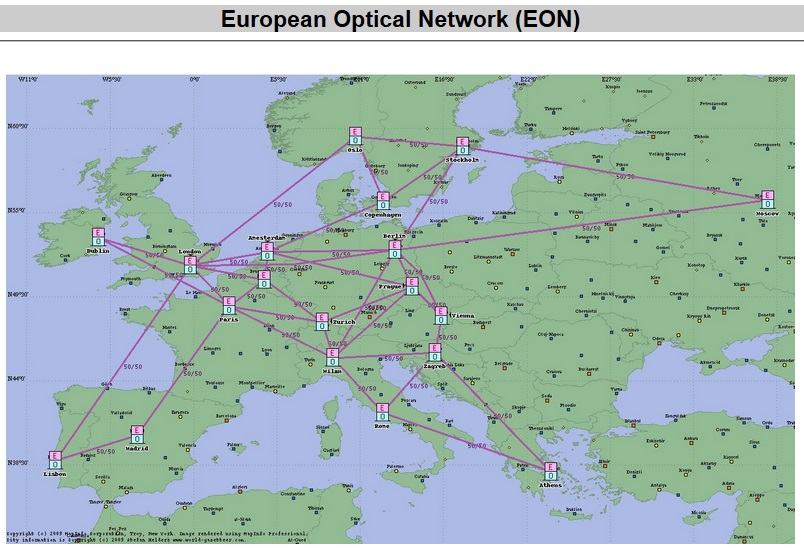
\includegraphics[width=\textwidth]{EON_Rede_Realista}
\caption{Physical Topology of the Realistic Network.}
\end{figure}

The table \ref{table:4} shows the values of the variables associated with this network.
\begin{table}[h!]
\centering
\begin{tabular}{|| c | c | c||}
 \hline
 Constant & Description & Value \\
 \hline\hline
 N & Number of nodes & 19 \\
 L & Number of bidirectional links & 37 \\
 <$\delta$> & Node out-degree & 3.89 \\
 <len> & Mean link length (km) & 753.76 \\
 <h> & Mean number of hops for working paths & 2.3 \\
 <h'> & Mean number of hops for backup paths & 3.2 \\
 \hline
\end{tabular}
\caption{Table of realistic network values}
\label{table:4}
\end{table}

Again, through the ODU's we can calculate the total traffic for both scenarios being them:
\begin{itemize}
  \item Low Traffic: \textbf{2 TBits/s}
  \item High Traffic: \textbf{20 TBits/s}
\end{itemize}


\[
  \text{Dist} = \kbordermatrix{
    & Oslo & Stockholm & Moscow & Copenhagen & Berlin & Prague & Vienna & Zagreb & Athens & Rome & Milan & Zurich & Brussels & Amesterdan & London & Dublin & Paris & Madrid & Lisbon \\
    Oslo & 0 & 500 & 500 & 0 & 0 & 0 & 0 & 500 & 500 & 0 & 0 & 500 & 500 & 0 & 0 & 0 & 0 & 500 & 500 \\
    Stockholm & 0 & 500 & 500 & 0 & 0 & 0 & 0 & 500 & 500 & 0 & 0 & 500 & 500 & 0 & 0 & 0 & 0 & 500 & 500 \\
    Moscow & 0 & 500 & 500 & 0 & 0 & 0 & 0 & 500 & 500 & 0 & 0 & 500 & 500 & 0 & 0 & 0 & 0 & 500 & 500 \\
    Copenhagen & 0 & 500 & 500 & 0 & 0 & 0 & 0 & 500 & 500 & 0 & 0 & 500 & 500 & 0 & 0 & 0 & 0 & 500 & 500 \\
    Berlin & 0 & 500 & 500 & 0 & 0 & 0 & 0 & 500 & 500 & 0 & 0 & 500 & 500 & 0 & 0 & 0 & 0 & 500 & 500 \\
    Prague & 0 & 500 & 500 & 0 & 0 & 0 & 0 & 500 & 500 & 0 & 0 & 500 & 500 & 0 & 0 & 0 & 0 & 500 & 500 \\
    Vienna & 0 & 500 & 500 & 0 & 0 & 0 & 0 & 500 & 500 & 0 & 0 & 500 & 500 & 0 & 0 & 0 & 0 & 500 & 500 \\
    Zagreb & 0 & 500 & 500 & 0 & 0 & 0 & 0 & 500 & 500 & 0 & 0 & 500 & 500 & 0 & 0 & 0 & 0 & 500 & 500 \\
    Athens & 0 & 500 & 500 & 0 & 0 & 0 & 0 & 500 & 500 & 0 & 0 & 500 & 500 & 0 & 0 & 0 & 0 & 500 & 500 \\
    Rome & 0 & 500 & 500 & 0 & 0 & 0 & 0 & 500 & 500 & 0 & 0 & 500 & 500 & 0 & 0 & 0 & 0 & 500 & 500 \\
    Milan & 0 & 500 & 500 & 0 & 0 & 0 & 0 & 500 & 500 & 0 & 0 & 500 & 500 & 0 & 0 & 0 & 0 & 500 & 500 \\
    Zurich & 0 & 500 & 500 & 0 & 0 & 0 & 0 & 500 & 500 & 0 & 0 & 500 & 500 & 0 & 0 & 0 & 0 & 500 & 500 \\
    Brussels & 0 & 500 & 500 & 0 & 0 & 0 & 0 & 500 & 500 & 0 & 0 & 500 & 500 & 0 & 0 & 0 & 0 & 500 & 500 \\
    Amesterdan & 0 & 500 & 500 & 0 & 0 & 0 & 0 & 500 & 500 & 0 & 0 & 500 & 500 & 0 & 0 & 0 & 0 & 500 & 500 \\
    London & 0 & 500 & 500 & 0 & 0 & 0 & 0 & 500 & 500 & 0 & 0 & 500 & 500 & 0 & 0 & 0 & 0 & 500 & 500 \\
    Dublin & 0 & 500 & 500 & 0 & 0 & 0 & 0 & 500 & 500 & 0 & 0 & 500 & 500 & 0 & 0 & 0 & 0 & 500 & 500 \\
    Paris & 0 & 500 & 500 & 0 & 0 & 0 & 0 & 500 & 500 & 0 & 0 & 500 & 500 & 0 & 0 & 0 & 0 & 500 & 500\\
    Madrid & 0 & 500 & 500 & 0 & 0 & 0 & 0 & 500 & 500 & 0 & 0 & 500 & 500 & 0 & 0 & 0 & 0 & 500 & 500 \\
    Lisbon & 0 & 500 & 500 & 0 & 0 & 0 & 0 & 500 & 500 & 0 & 0 & 500 & 500 & 0 & 0 & 0 & 0 & 500 & 444
  }
\]


\newpage
\subsection{Dimensioning using ILP}
\begin{tcolorbox}	
\begin{tabular}{p{2.75cm} p{0.2cm} p{10.5cm}} 	
\textbf{Student Name}  &:& Tiago Esteves    (October 03, 2017 - )\\
\textbf{Goal}          &:& Implement the dimensioning of optical networks in the transparent transport mode.
\end{tabular}
\end{tcolorbox}

\subsubsection{ILP Models} \label{ILP_models_Transp}

Again, for a better understanding of the functions and variables used in the ILP, a table \ref{description_transp} will be created with all the variables and their description. \\

\begin{table}[h!]
\centering
\begin{tabular}{ |p{1cm}||p{13cm}|}
 \hline
 \multicolumn{2}{|c|}{Description of notation used in the objective function} \\
 \hline
 \hline
 $i$ & index for start node of a physical link \\
 $j$ & index for end node of a physical link \\
 $o$ & index for node that is origin of a demand \\
 $d$ & index for node that is destination of a demand \\
 $($ i,j $)$ & physical link between the nodes $i$ and $j$ \\
 $($ o,d $)$ & demand between the nodes $o$ and $d$ \\
 $f_{ij}^{od}$ & Number of 100 Gbit/s optical channels (number of flows) between the link $i$ and $j$ for all demand pairs between $o$ and $d$ \\
 $W_{od}$ & number of optical channels between the nodes $o$ and $d$\\
 G & Network topology in form of adjacency matrix \\
 \hline
\end{tabular}
\caption{Table with description of variables}
\label{description_transp}
\end{table}


The optimization model suggested for transparent transport mode with dedicated path protection intends to minimize the total number of flows crossing link (i, j) for all demand pairs (o, d). The mathematical model described below also minimizes the total number of optical channels between each demand end nodes $W_{od}$, instead of minimizing the number of optical link-by-link channels as in the previous model.

\vspace{10pt}
\begin{equation}
minimize    \sum_{(i,j)} \sum_{(o,d)} f_{ij}^{od} + \sum_{(o,d)} W_{od}
\label{ILPTransp}
\end{equation}

$subject$ $to$
\begin{equation}
\sum_{j\textbackslash \{o\}} f_{ij}^{od} = 2  \qquad \qquad \qquad \qquad \qquad \qquad \qquad \qquad \qquad \qquad
\forall(o,d) : o < d, \forall i: i = o
\label{ILPTransp1}
\end{equation}

\begin{equation}
\sum_{j\textbackslash \{o\}} f_{ij}^{od} = \sum_{j\textbackslash \{d\}} f_{ji}^{od}   \qquad \qquad \qquad \qquad \qquad \qquad \qquad \qquad
\forall(o,d) : o < d, \forall i: i \neq o,d
\label{ILPTransp2}
\end{equation}

\begin{equation}
\sum_{j\textbackslash \{d\}} f_{ji}^{od} = 2  \qquad \qquad \qquad \qquad \qquad \qquad \qquad \qquad \qquad \qquad
\forall(o,d) : o < d, \forall i: i = d
\label{ILPTransp3}
\end{equation}

\begin{equation}
\sum_{(o,d):o<d} \left(f_{ij}^{od} + f_{ji}^{od}\right) W_{od} \leq 80 G_{ij} \qquad \qquad \qquad \qquad \qquad \qquad \qquad \qquad
\forall(i,j) : i < j
\label{ILPTransp4}
\end{equation}

\begin{equation}
f_{ij}^{od} , f_{ji}^{od} \in \{0,2\}   \qquad \qquad \qquad \qquad \qquad \qquad \qquad \qquad \qquad
\forall(i,j) : i < j, \forall(o,d) : o < d
\label{ILPTransp5}
\end{equation}

\begin{equation}
W_{od} \in \mathbb{N}  \qquad \qquad \qquad \qquad \qquad \qquad \qquad \qquad \qquad \qquad \qquad \qquad \qquad
\forall(o,d) : o < d
\label{ILPTransp6}
\end{equation}


The objective function, to be minimized, is the expression \ref{ILPTransp}. The flow conservation is performed by equations \ref{ILPTransp1}, \ref{ILPTransp2} and \ref{ILPTransp3} and share the same mathematical description of opaque model. The inequality \ref{ILPTransp4} answers capacity constraint problem. Then, total flows times the traffic of the demands must be less or equal to the capacity of network links. The grooming of this model can be done before routing since the traffic is aggregated just for demands between the same nodes, thus not depending on the routes. Last two constraints define the total number of flows must be zero if there is no demand, or two for a demand with traffic protection, and the number of optical channels must be a counting number.

\subsubsection{ILP Results}

In this initial phase the results will be presented using ILP to calculate the CAPEX of the reference network and the realistic network.
The value of the CAPEX of the network will be calculated based on the costs of the equipment present in the table below.

\begin{table}[h!]
\centering
\begin{tabular}{|| c | c||}
 \hline
 Equipment & Cost \\
 \hline\hline
 OLT without transponders & 15000 \euro \\
 Transponder & 5000 \euro/Gb \\
 Optical Amplifier & 4000 \euro \\
 EXC & 10000 \euro \\
 OXC & 20000 \euro \\
 EXC Port & 1000 \euro /Gb/s\\
 OXC Port & 2500 \euro /porto \\
 \hline
\end{tabular}
\caption{Table with costs}
\label{table_cost2}
\end{table}

In addition to the equipment costs we will also use the parameter "span", which in this case will have a value of 100, because this value is used to calculate the number of optical amplifiers required in the network using Equation \ref{amplifiersTransp}.

\begin{equation}
N^R = \sum\limits_{l=1}^L\left(\left\lceil\frac{len_l}{span}\right\rceil-1\right)
\label{amplifiersTransp}
\end{equation} \\

To know the value of CAPEX it is necessary to know the value of the cost of the links and the cost of the nodes.

To calculate the cost of the nodes, the sum of the costs of the optical and electrical node is made. For this case the optical cost is given by equation \ref{opticalCost} and the electrical cost by the equation \ref{electricalCostTransp}.


\begin{equation}
C_{oxc} = \left(\gamma_{o0} \times N \right) + \gamma_{o1} \times  \left(P_{LINE} + P_{ADD}\right)
\label{opticalCost}
\end{equation}	
	
\begin{itemize}
\item{$C_{oxc}$		$\rightarrow$	Optical Ports Cost}
\item{$\gamma_{o0}$	$\rightarrow$	OXC cost in Euros}
\item{$\gamma_{o1}$	$\rightarrow$	OXC port cost in Euros}
\item{$P_{TRIB}	$	$\rightarrow$	Number of tributary ports}
\item{$P_{ADD} $	$\rightarrow$	Number of adding ports}
\end{itemize}

\begin{equation}
C_{exc} = \left(\gamma_{e0}\times N\right) + \gamma_{e1} \times \left(2 \times T_1 \right)		\label{electricalCostTransp}
\end{equation}

\vspace{10pt}

To calculate the cost of the Links we will use the equation \ref{linkCostsTransp}.

\begin{equation}
C_L = \left(2 \times \gamma_0^{OLT} \times L\right) + \left(2 \times \gamma_1^{OLT} \times \tau \times W\right) + \left(N^R \times c^R\right)
\label{linkCostsTransp}
\end{equation} \\
	
\vspace{11pt}
To perform the calculations using the implementation of the models described in section \ref{ILP_models_OP} it is necessary to use a mathematical software tool. For this we will use MATLAB which is ideal for dealing with linear programming problems and can call the LPsolve through an external interface. \\

\textbf{Scenario 1: Test Network Low Traffic} \label{Scenario1_transp} \\
In this scenario we used the table \ref{table:3}. In the table \ref{result_ILP1_T} we can see the values calculated through MatLab and using the values indicated in table \ref{table_cost2} we can finally calculate the CAPEX value. \\
\newpage
\begin{table}[h!]
\centering
\begin{tabular}{|| c | c||}
 \hline
 Number of optical channels & Value \\
 \hline\hline
 in the link (1,2) & 2 \\
 in the link (1,3) & 2 \\
 in the link (2,3) & 4 \\
 in the link (2,4) & 3 \\
 in the link (3,5) & 3 \\
 in the link (4,5) & 3 \\
 in the link (4,6) & 3 \\
 in the link (5,6) & 3 \\
 \hline
\end{tabular}
\caption{Table with results}
\label{result_ILP1_T}
\end{table}

Using equation \ref{linkCostsTransp} : \\
$C_L$ = $($2 * 15 000 * 8$)$ + $($2 * 5 000 * 100 * $)$ + $($24 * 4 000$)$ \\
$C_L$ = \textbf{ \euro} \\

Using equation \ref{electricalCostTransp} : \\
$C_{exc}$ = $($6 * 10 000$)$ + 1 000 * $($2 * 1 000$)$ \\
$C_{exc}$ = \textbf{2 060 000\euro} \\

Using equation \ref{opticalCost} : \\
$C_{oxc}$ = $($6 * 10 000$)$ + 1 000 * $($ + $)$ \\
$C_{oxc}$ = \textbf{ \euro} \\
$C_N$ = $C_{oxc}$ + $C_{exc}$ = \textbf{ \euro} \\

$CAPEX$ =  +  = \textbf{ \euro}\\

\textbf{Scenario 2: Test Network High Traffic} \label{Scenario2_transp} \\
In this scenario we used again the table \ref{table:3} In the table \ref{result_ILP2_T} we can see the values calculated through MatLab and using the values indicated in table \ref{table_cost2} we can finally calculate the CAPEX value.

\begin{table}[h!]
\centering
\begin{tabular}{|| c | c||}
 \hline
 Number of optical channels & Value \\
 \hline\hline
 in the link (1,2) & 2 \\
 in the link (1,3) & 2 \\
 in the link (2,3) & 4 \\
 in the link (2,4) & 3 \\
 in the link (3,5) & 3 \\
 in the link (4,5) & 3 \\
 in the link (4,6) & 3 \\
 in the link (5,6) & 3 \\
 \hline
\end{tabular}
\caption{Table with results}
\label{result_ILP2_T}
\end{table}


Using equation \ref{linkCostsTransp} : \\
$C_L$ = $($2 * 15 000 * 8$)$ + $($2 * 5 000 * 100 * $)$ + $($24 * 4 000$)$ \\
$C_L$ = \textbf{ \euro} \\

Using equation \ref{electricalCostTransp} : \\
$C_{exc}$ = $($6 * 10 000$)$ + 1 000 * $($2 * 2 000$)$ \\
$C_{exc}$ = \textbf{4 060 000 \euro} \\

Using equation \ref{opticalCost} : \\
$C_{oxc}$ = $($6 * 10 000$)$ + 1 000 * $($ + $)$ \\
$C_{oxc}$ = \textbf{ \euro} \\
$C_N$ = $C_{oxc}$ + $C_{exc}$ = \textbf{ \euro} \\

$CAPEX$ =  +  = \textbf{ \euro}\\


\vspace{11pt}
\textbf{Scenario 3: Realistic Network Low Traffic} \label{Scenario3_transp} \\
In this scenario we used the table \ref{table:4} In the table \ref{result_ILP3_T} we can see the values calculated through MatLab and using the values indicated in table \ref{table_cost2} we can finally calculate the CAPEX value. \\

\begin{table}[h!]
\centering
\begin{tabular}{|| c | c||}
 \hline
 Number of optical channels & Value \\
 \hline\hline
 in the link (1,2) & 2 \\
 in the link (1,3) & 2 \\
 in the link (2,3) & 4 \\
 in the link (2,4) & 3 \\
 in the link (3,5) & 3 \\
 in the link (4,5) & 3 \\
 in the link (4,6) & 3 \\
 in the link (5,6) & 3 \\
 \hline
\end{tabular}
\caption{Table with results}
\label{result_ILP3_T}
\end{table}

Using equation \ref{linkCostsTransp} : \\
$C_L$ = $($2 * 15 000 * 37$)$ + $($2 * 5 000 * 100 * $)$ + $($24 * 4 000$)$ \\
$C_L$ = \textbf{ \euro} \\

Using equation \ref{electricalCostTransp} : \\
$C_{exc}$ = $($19 * 10 000$)$ + 1 000 * $($2 * 4 000$)$ \\
$C_{exc}$ = \textbf{8 190 000\euro} \\

Using equation \ref{opticalCost} : \\
$C_{oxc}$ = $($19 * 10 000$)$ + 1 000 * $($ + $)$ \\
$C_{oxc}$ = \textbf{ \euro} \\
$C_N$ = $C_{oxc}$ + $C_{exc}$ = \textbf{ \euro} \\

$CAPEX$ =  +  = \textbf{ \euro}\\


\vspace{11pt}
\textbf{Scenario 4: Realistic Network High Traffic} \label{Scenario4_transp} \\
In this scenario we used again the table \ref{table:4} In the table \ref{result_ILP4_T} we can see the values calculated through MatLab and using the values indicated in table \ref{table_cost2} we can finally calculate the CAPEX value. \\

\begin{table}[h!]
\centering
\begin{tabular}{|| c | c||}
 \hline
 Number of optical channels & Value \\
 \hline\hline
 in the link (1,2) & 2 \\
 in the link (1,3) & 2 \\
 in the link (2,3) & 4 \\
 in the link (2,4) & 3 \\
 in the link (3,5) & 3 \\
 in the link (4,5) & 3 \\
 in the link (4,6) & 3 \\
 in the link (5,6) & 3 \\
 \hline
\end{tabular}
\caption{Table with results}
\label{result_ILP4_T}
\end{table}

Using equation \ref{linkCostsTransp} : \\
$C_L$ = $($2 * 15 000 * 37$)$ + $($2 * 5 000 * 100 * $)$ + $($24 * 4 000$)$ \\
$C_L$ = \textbf{ \euro} \\

Using equation \ref{electricalCostTransp} : \\
$C_{exc}$ = $($19 * 10 000$)$ + 1 000 * $($2 * 40 000$)$ \\
$C_{exc}$ = \textbf{80 190 000\euro} \\

Using equation \ref{opticalCost} : \\
$C_{oxc}$ = $($19 * 10 000$)$ + 1 000 * $($ + $)$ \\
$C_{oxc}$ = \textbf{ \euro} \\
$C_N$ = $C_{oxc}$ + $C_{exc}$ = \textbf{ \euro} \\

$CAPEX$ =  +  = \textbf{ \euro}\\

\newpage

\subsection{Dimensioning using Heuristics}

\subsubsection{Heuristics Models}

\subsubsection{Heuristics Results}

\subsection{Comparative Analysis} 
\clearpage

\begin{tcolorbox}	
\begin{tabular}{p{2.75cm} p{0.2cm} p{10.5cm}} 	
\textbf{Student Name}  &:& Tiago Esteves\\
\textbf{Starting Date} &:& October 03, 2017\\
\textbf{Goal}          &:& Implement the dimensioning of optical networks in the translucent transport mode.
\end{tabular}
\end{tcolorbox}

\section{Translucent with 1+1 Protection}
In this case study we focus on the translucent case with 1 + 1 protection.


\subsection{Physical Network Topology}

\subsubsection{Reference Network}
As we can see in the figure, our reference network consists of 6 nodes and 8 Bidirectional links.
The average length of the links was chosen so that the following calculations are more simplistic.

\begin{figure}[h!]
\centering
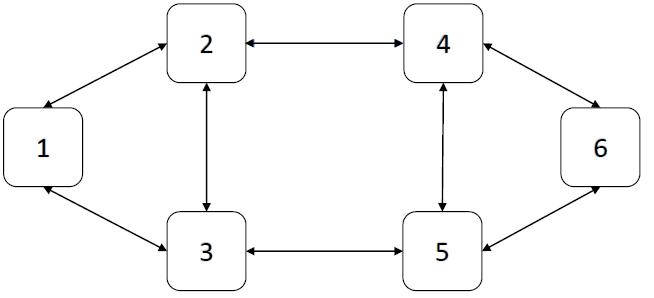
\includegraphics[width=\textwidth]{RedeTeste}
\caption{Physical Topology of the Reference Network.}
\end{figure}

The following table shows the values of the variables associated with this network.
\begin{table}[h!]
\centering
\begin{tabular}{|| c | c | c||}
 \hline
 Constant & Description & Value \\
 \hline\hline
 N & Number of Nodes & 6 \\
 L & Number of Bidirectional Links & 8 \\
 <$\delta$> & Node out-degree & 2,667 \\
 <len> & Mean Link Length (km) & 500 \\
 <h> & Mean Number of Hops,for Working Paths & 1,533 \\
 <h'> & Mean Number of Hops,for Backup Paths & 2,467 \\
 \hline
\end{tabular}
\caption{Table of reference network values}
\label{table:5}
\end{table}

As we can see from table \ref{table:5}, to do all the calculations necessary for this project, let us know the value of the traffic used. This value is defined depending on the scenario used, as we can see:
\begin{itemize}
  \item Low Traffic: \textbf{0.5 TBits/s}
  \item High Traffic: \textbf{5 TBits/s}
\end{itemize}

\subsubsection{Realistic Network}
The real network chosen for this work is the EON (European Optical Network). \\
The way the nodes are arranged geographically can be seen from the following figure.

\begin{figure}[h!]
\centering
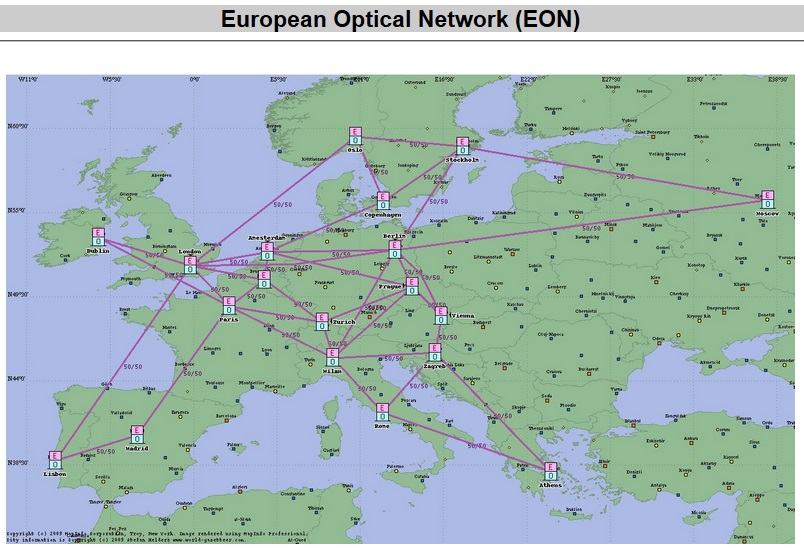
\includegraphics[width=\textwidth]{EON_Rede_Realista}
\caption{Physical Topology of the Realistic Network.}
\end{figure}


Again, to make all the necessary calculations, only the value of the traffic used is missing. This value is set depending on the scenario used, as we can see:

\begin{itemize}
  \item Low Traffic: \textbf{2 TBits/s}
  \item High Traffic: \textbf{20 TBits/s}
\end{itemize}

\begin{table}[h!]
The table \ref{table:6} shows the values of the variables associated with this network.\vspace{10pt}
\centering
\begin{tabular}{|| c | c | c||}
 \hline
 Constant & Description & Value \\
 \hline\hline
 N & Number of Nodes & 19 \\
 L & Number of Bidirectional Links & 37 \\
 <$\delta$> & Node out-degree & 3,89 \\
 <len> & Mean Link Length (km) & 753,76 \\
 <h> & Mean Number of Hops,for Working Paths & 2,3 \\
 <h'> & Mean Number of Hops,for Backup Paths & 3,2 \\
 \hline
\end{tabular}
\caption{Table of realistic network values}
\label{table:6}
\end{table}

\newpage
\subsection{Dimensioning using ILP}

\subsubsection{ILP models} \label{ILP_models_Transluc}

Again, for a better understanding of the functions and variables used in the ILP, a table \ref{description_transluc} will be created with all the variables and their description. \\

\begin{table}[h!]
\centering
\begin{tabular}{|| c | c||}
 \hline
 Variables & Description \\
 \hline\hline
 $($ i,j $)$ & Origin node, i and destination node, j of a Link \\
 $($ o,d $)$ & Origin node, o and destination node, d of a Demand \\
 c & Client traffic Type $($ 1 to 5 $)$ \\
 L &  \\
 y &  \\
 W & Number of optical channels \\
 B & Client signals granularities $($1.25, 2.5, 10, 40, 100$)$ \\
 D & Client traffic demands \\
 G & Network topology in form of Adjacency matrix \\
 BD & \\
 \hline
\end{tabular}
\caption{Table with description of variables}
\label{description_transluc}
\end{table}

\vspace{20pt}

\begin{equation}
minimize \qquad \qquad \qquad \qquad \qquad  \sum_{(o,d,b)} W_{od}
\label{ILPTransluc}
\end{equation}

$subject$ $to$

\begin{equation}
\sum_{j \neq i} L_{ij}^{od} = D_{odc}
\qquad \qquad \qquad \qquad \qquad \qquad \qquad \qquad \qquad
\forall o,c,d : o < d
\label{ILPTransluc1}
\end{equation}

\begin{equation}
\sum_{j \neq i \ j \neq o} L_{ij}^{od} = \sum_{j \neq i \ j \neq o} L_{ji}^{od}
\qquad \qquad \qquad \qquad \qquad \qquad
\forall s,d,p,o : s < d : p \neq s : p \neq d
\label{ILPTransluc2}
\end{equation}

\begin{equation}
\sum_{i \neq j} L_{ji}^{od} = D_{odc}
\qquad \qquad \qquad \qquad \qquad \qquad \qquad \qquad
\forall o,d,c : o < d
\label{ILPTransluc3}
\end{equation}

\begin{equation}
\sum_{(o,d,c): o<d} (B(c) \times L_{ij}^{od}) \leq  \sum_{b} BD_b \times W_{ijb}
\qquad \qquad \qquad \qquad \qquad
\forall i,j
\label{ILPTransluc4}
\end{equation}

\begin{equation}
L_{ij}^{od} \geq 0;
\qquad \qquad \qquad \qquad \qquad \qquad \qquad \qquad \qquad \qquad
\forall o,d,i,j : o < d
\label{ILPTransluc5}
\end{equation}

\begin{equation}
\sum_{i \neq j} y_{ij}^{od} = W_{od}
\qquad \qquad \qquad \qquad \qquad \qquad \qquad \qquad \qquad \qquad \qquad
\forall i,j,b
\label{ILPTransluc6}
\end{equation}

\begin{equation}
\sum_{j\neq i \ j\neq o} y_{ij}^{od} = \sum_{j \neq i \ j \neq d} y_{ji}^{od}
\qquad \qquad \qquad \qquad \qquad \qquad \qquad
\forall o,d,i,b : i \neq d : i \neq o
\label{ILPTransluc7}
\end{equation}

\begin{equation}
\sum_{j \neq i} y_{ji}^{od} = W_{od}
\qquad \qquad \qquad \qquad \qquad \qquad \qquad \qquad \qquad \qquad \qquad
\forall o,d,b
\label{ILPTransluc8}
\end{equation}

\begin{equation}
\sum_{(o,d,b)} \left( y_{ij}^{od} + y_{ji}^{od}\right) \leq 80 G_{ij}
\qquad \qquad \qquad \qquad \qquad \qquad \qquad
\forall i,j : i < j
\label{ILPTransluc9}
\end{equation}

\begin{equation}
y_{ij}^{od} \geq 0
\qquad \qquad \qquad \qquad \qquad \qquad \qquad \qquad \qquad \qquad \qquad \qquad
\forall o,d,i,j,b
\label{ILPTransluc10}
\end{equation}	


\subsubsection{ILP Results}

In this initial phase the results will be presented using ILP to calculate the CAPEX of the reference network.

The value of the CAPEX of the network will be calculated based on the costs of the equipment present in the table below.
\begin{table}[h!]
\centering
\begin{tabular}{|| c | c||}
 \hline
 Equipment & Cost \\
 \hline\hline
 OLT without transponders & 15000 \euro \\
 Transponder & 5000 \euro/Gb \\
 Optical Amplifier & 4000 \euro \\
 EXC & 10000 \euro \\
 OXC & 20000 \euro \\
 EXC Port & 1000 \euro /Gb/s\\
 OXC Port & 2500 \euro /porto \\
 \hline
\end{tabular}
\caption{Table with costs}
\label{table_cost3}
\end{table}

In addition to the equipment costs, we will also use the parameter "span", which in this case will have a value of 100.
Because this value is used to calculate the number of optical amplifiers required in the network using Equation \ref{amplifiersTranslu}.

\begin{equation}
N^R = \sum\limits_{l=1}^L\left(\left\lceil\frac{len_l}{span}\right\rceil-1\right)
\label{amplifiersTranslu}
\end{equation} \\

To know the value of CAPEX it is necessary to know the value of the cost of the links and the cost of the nodes.

To calculate the cost of the nodes, the sum of the costs of the optical and electrical node is made. %For this case the optical cost is given by equation \ref{opticalCost} and the electrical cost by the equation \ref{electricalCostTransp}.

%\begin{equation}
%C_{oxc} = \left(\gamma_{o0} \times N \right) + \gamma_{o1} \times  \left(P_{LINE} + P_{ADD}\right)
%\label{opticalCost}
%\end{equation}	
	
%\begin{itemize}
%\item{$C_{oxc}$		$\rightarrow$	Optical Ports Cost}
%\item{$\gamma_{o0}$	$\rightarrow$	OXC cost in Euros}
%\item{$\gamma_{o1}$	$\rightarrow$	OXC port cost in Euros}
%\item{$P_{TRIB}	$	$\rightarrow$	Number of tributary ports}
%\item{$P_{ADD} $	$\rightarrow$	Number of adding ports}
%\end{itemize}

%\begin{equation}
%C_{exc} = \left(\gamma_{e0}\times N\right) + \gamma_{e1} \times \left(2 \times T_1 \right)		\label{electricalCostTransp}
%\end{equation} \\


To calculate the cost of the Links we will use the equation .

%\begin{equation}
%C_L = \left(\gamma_0^{OLT} \times L\right) + \left(\gamma_1^{OLT} \times \tau \times W\right) + \left(N^R \times %c^R\right)
%\label{linkCostsTransp}
%\end{equation} \\
	

Finally we will calculate the CAPEX values for the various situations mentioned.\\

\textbf{Low Traffic scenario:}\\

$C_L$ = \textbf{\euro}

$C_N$ = \textbf{\euro}

$CAPEX$ = \textbf{\euro}\\

\textbf{High Traffic scenario:}\\

$C_L$ = \textbf{\euro}

$C_N$ = \textbf{ \euro}

$CAPEX$ =  \textbf{ \euro}\\

\subsection{Dimensioning using Analytical solution}

\subsubsection{Analytical Models}

\subsubsection{Analytical Results}

\newpage

\subsection{Dimensioning using Heuristics}

\subsubsection{Heuristics Models}

\subsubsection{Heuristics Results}

\subsection{Analysis and comparison of results}





%\section{Continuous Variable Quantum Transmission System}
%
%\subfile{./sdf/cv_system/cv_system}


%\include{sdf/cv_system/cv_system}
%\include{../sdf/TexFiles/EnquadramentoVHDL}
%\include{CapacidadeTeoriacadeTransmitirInformacao}
%\include{SistemasCoerentesComDSP}
%\include{SistemasMultiMode}
%\include{SistemasComunicacaoQuanticos}
%\include{Conclusao}
%\appendix
%\include{Acronymous}
%\printindex

%   create the appendix and include it


\pagebreak

%--------------------------------- SECTION ----------------------------------
\bibliographystyle{ieeetr}
% argument is your BibTeX string definitions and bibliography database(s)
%\bibliography{../../../Computadores/Bibtex/IEEEabrv,../../../Computadores/Bibtex/AnpBib}


\printglossaries

\end{document}
